\documentclass{article}
\usepackage{graphicx} % Required for inserting images
\usepackage{amsthm}
\usepackage{amsmath}   % Core math formatting
\usepackage{amssymb}   % Provides symbols (like \mathbb, \checkmark)
\usepackage{amsfonts}  % More math fonts
\usepackage{mathptmx}
\newcommand{\qed}{\hfill $\square$}
\title{Convex Optimization - Exercises from Chapter 3 of Boyd}
\author{Kontovrakis Konstantinos}
\date{February 2026}

\begin{document}

\maketitle

\section*{2.2}

 A set $S$ is convex if and only if its intersection with any line is convex.


 First, we will show one way. If the set $S$ is convex, then the intersection with any line $L$ is convex. This is simple because we know that the intersection of any two convex sets is a convex set, and a line is a convex set by definition.

 To show the other way, suppose the intersection of a set $S$ with any line is convex. Say we have two points in the set $S$: $x_1, x_2$. There is a line $L$ that connects these two points. The intersection $S \cap L$ is convex, which means that it contains all the convex combinations of the two points $x_1$ and $x_2$. Since the combinations are in the intersection, this means that they are also in the set $S$. This means that all the convex combinations of the two points are in the set; thus, the set $S$ is convex. 

We have shown both ways.


\medskip
 A set $S$ is affine if and only if its intersection with any line is affine.
 First, we will show one way. If the set $S$ is affine, then the intersection with any line $L$ is affine. This is simple because we know that the intersection of any two affine sets is an affine set, and a line is an affine set by definition.

 
 To show the other way, suppose the intersection of a set $S$ with any line is affine. Say we have two points in the set $S$: $x_1, x_2$. There is a line $L$ that connects these two points. The intersection $S \cap L$ is affine, which means that it contains all the affine combinations of the two points $x_1$ and $x_2$. Since the combinations are in the intersection, this means that they are also in the set $S$. This means that all the affine combinations of the two points are in the set; thus, the set $S$ is affine. 

We have shown both ways.






\newpage


\section*{2.4}

The convex hull of a set S is the intersection of all convex sets that contain S. 

Let \textbf{S} be a set. H = \textbf{conv} \textbf{S} the convex hull of the set \textbf{S}. Let \textbf{I} be the intersection of all convex sets C that contain \textbf{S}.

We prove that H=I , by showing that $H \subseteq I   $  and $I \subseteq H   $  .

First, because I is the intersection of all convex sets that include S , and  H is a convex set that includes S, it is proven that  $I \subseteq H   $ .   

Second, to show that $H \subseteq I   $ , we suppose that we have one of the convex sets that make up I. Let $x_1 , x_2 , x_3 , ... ,x_n $be points in S . Because the set C is convex, and contains S, the convex combination of these points is included in the set.
Because I is the intersection of any such set C, it means that every set C must include the convex combinations of these points. This means that the intersection is made up only by the convex combination of such points. This means that $H \subseteq I$.


Since we showed both ways, we have shown that H=I.






\newpage

\section*{2.8}
A polyhedron is a set defined by a finite number of linear inequalities and linear equalities:
\[
P = \{x \mid Fx \preceq c,\; Gx = d\}.
\]



\textbf{(a)}
 $S = \{y_1 a_1 + y_2 a_2 \mid -1 \le y_1 \le 1, -1 \le y_2 \le 1\}$




 
 The set $S$ is a polyhedron.

 
 $S$ is the image of the unit square $C = \{y \in \mathbb{R}^2 \mid -1 \le y_1 \le 1, -1 \le y_2 \le 1\}$ under the linear transformation  $ Ay$, where $A = [a_1 \ a_2] \in \mathbb{R}^{n \times 2}$.
 
 As the image of a square under a linear mapping, $S$ is a parallelogram (or a line segment/point if $a_1, a_2$ are linearly dependent).


Since the unit square $C$ is a polytope and the image of a polytope under a linear mapping is also a polytope, $S$ is a polytope.









\textbf{(b)} 
We have generalized inequalities of this form : 
\[ x\succeq 0  \]

and if we write : 
\[a^T = [a_1 , ... ,a_n]\]

and 

\[b^T=[a_1^2,...,a_n^2]\]

,
then the sums that define the set can be written as :
\[a^Tx = b_1  \ and \ b^Tx = b_2 \]



Thus this set is a polyhedron.



\textbf{(c)} 
Our set  : S = \{ x \in \mathbb{R}^n \mid x \succeq 0,\; x^T y \le 1 \text{ for all } y \text{ with } \|y\|_2 = 1 \}

We rewrite the inequality as follows : 


\[|x^T y| \leq ||x||*||y||\ = ||x|| \leq1    \]
We used the Cauchy-Swartz inequality, and the conditions that define the set for this derivation ($||y||=1 \ and \ x^Ty\leq 1$).
This means that this inequality defines the unit ball. 
Our set is also only elements from the non-negative orthant $(x\succeq0)$ . 
We need an infinite number of linear solutions to write this set.
Thus the set is not a polyhedron.





\textbf{(d)} The set is $S = \{ x \in \mathbb{R}^n \mid x \succeq 0, \; x^T y \le 1 

The set $S$ is a polyhedron.
 The condition $x^T y \le 1$ for all $y$ such that $\|y\|_1 = 1$ is equivalent to $x_i \le 1$ for all $i = 1, \dots, n$.
By testing the specific unit vectors $y = e_i$ (where $\|e_i\|_1 = 1$), the condition $x^T e_i \le 1$ implies $x_i \le 1$ for each 

If $0 \le x_i \le 1$, then for any $y$ with $\sum |y_i| = 1$, we have $\sum x_i y_i \le \sum 1 \cdot |y_i| = 1$.
 The set $S$ is defined by $2n$ linear inequalities:
    \[ 0 \le x_i \le 1, \quad i = 1, \dots, n \]
$S$ is a bounded intersection of a finite number of halfspaces , which is a polyhedron.









\newpage

\section*{2.23}

Example of two closed convex sets, that are disjoint but cannot be strictly separated. \\

Set 1 : \[S_1 = \{ (x,y) | y \leq 0 \}\]  \\
Set 2 : \[S_2 = \{ (x,y) | y \geq e^{-x} , x,y \in \mathbf{R}    \}\]


\begin{figure}[h]
    \centering
    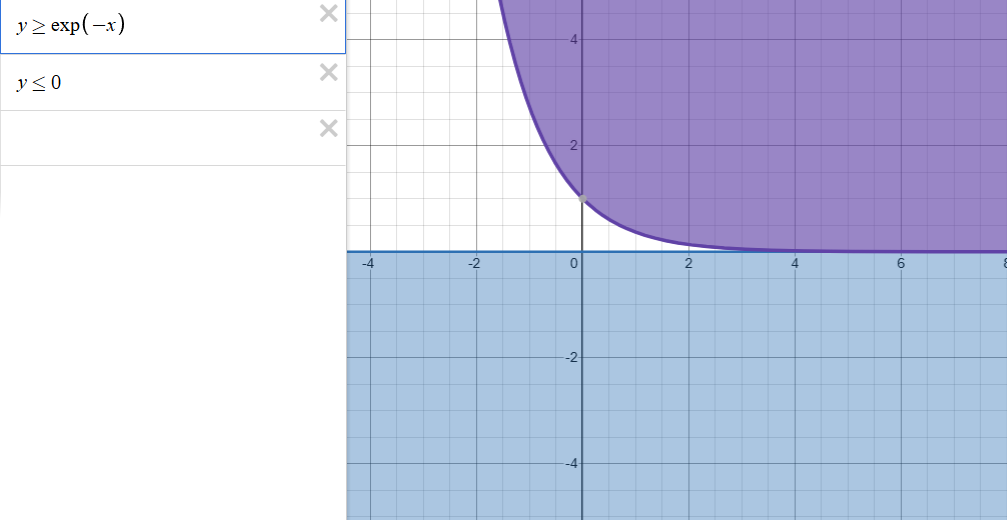
\includegraphics[width=1\linewidth]{separated.png}
    \caption{The sets $y \leq 0$ and $y \geq e^{-x}$ approach each other as $x \to \infty$, preventing strict separation.}
    \label{fig:placeholder}
\end{figure}






\newpage

\section*{2.16}
 If two sets are convex in $\mathbf{R^{mxn}}$, so is their partial sum.
 \[S = \{ (x, y_1 + y_2) \mid x \in \mathbf{R}^m, y_1, y_2 \in \mathbf{R}^n, (x, y_1) \in S_1, (x, y_2) \in S_2 \} \]





$S_1, S_2$ convex


Let $(x, y_1), (x', y_1') \in S_1$ \\
and $(x, y_2), (x', y_2') \in S_2$

Also: 
\[ (x, y_1 + y_2), (x', y_1' + y_2') \in S \]

We show that the convex combination of two elements of $S$ \\
are included in $S$.

\[ \theta (x, y_1 + y_2) + (1 - \theta) (x', y_1' + y_2') = \] \[ (\theta x + (1 - \theta) x', \theta y_1 + (1 - \theta) y_1' + \theta y_2 + (1 - \theta) y_2') \]

We see that this is the partial sum of \\
the elements:
\[ (\theta x + (1 - \theta) x', \theta y_1 + (1 - \theta) y_1') \in S_1 \]
and
\[ (\theta x + (1 - \theta) x', \theta y_2 + (1 - \theta) y_2') \in S_2 \]

They are convex combinations of \\
$(x, y_i)$ and $(x', y_i')$ \\
which means they are elements of $S_1$ and $S_2$ respectively because they are convex sets.

We have shown that the convex combination of 2 elements \\
of the partial sum is also in partial sum.


























\newpage
\section*{2.12}
\textbf{(a)} As an intersection of  2 halfspaces, a slab is convex : \[ \{ x\in \mathbf{R}^n | \alpha \leq a^Tx \}\cap   \{ x\in \mathbf{R}^n |  a^Tx \leq  \beta\} \]


\\
\textbf{(b)} It is the intersection of many halfspaces. We can think of the confinement in each dimension , as a slab. The intersection of all these constraints creates the rectangle. Because it is the intersection of convex sets, it is convex. 

\\

\textbf{(c)} This is the intersection of and \[\{x \in \mathbf{R^n} | a^T
1x \leq b1 \} \\ \cap \\  \{x \in \mathbf{R^n} | a^T
2x \leq b2\} \]
These are two halfspaces. Halfspaces are convex. This is the intersection of two halfspaces. Thus the set is convex.

\textbf{(d)} For a given y of the set $S$ we can rewrite the inequality in another form and show it is a halfspace. 
Because the Euclidean norm is non-negative , if we square the inquality, it still holds.
Set of points close to a given point than a given set :
\[
D = \{ x \mid \|x - x_0\|^2 \le \|x - y\|^2 \ \text{for all } y \in S \}
\]

We simplify the inequality : 
\begin{align*}
\|x - x_0\|_2^2 &\leq \|x - y\|_2^2 \\
(x - x_0)^T (x - x_0) &\leq (x - y)^T (x - y) \\
(x^T - x_0^T)(x - x_0) &\leq (x^T - y^T)(x - y) \\
x^T x - x_0^T x - x^T x_0 + x_0^T x_0 &\leq x^T x - x^T y - y^T x + y^T y \\
-x_0^T x - x^T x_0 + x_0^T x_0 &\leq -x^T y - y^T x + y^T y \\
y^T x - x_0^T x - x^T x_0 + x^T y &\leq -x_0^T x_0 + y^T y \\
(y^T - x_0^T)x + x^T(y - x_0) &\leq \|y\|_2^2 - \|x_0\|_2^2 \\
(y - x_0)^T x + x^T(y - x_0) &\leq y^T y - x_0^T x_0 \\ 
\text{$(y-x_0)^Tx$ is a scalar and equal to its transpose} \\ 
2 (y - x_0)^T x &\leq y^T y - x_0^T x_0 \\
\end{align*}

For a given y, the set of points for which this inequality holds is a halfspace.

We can rewrite the  original set D as an intersection of halfspaces of the former form, for all possible values of y. 

\[D = \{ x \mid \|x - x_0\|^2 \le \|x - y\|^2 \ \text{for all } y \in S \} = \bigcap_{y\in S}\{ x \mid \|x - x_0\|^2 \le \|x - y\|^2 \ \} \]

Because it is an intersection of halfspaces which are convex, our set D is convex.


\newpage
\textbf{(e)} The set $D = \{x \mid \text{dist}(x,S) \le \text{dist}(x,T)\}$ is not necessarily convex and we prove this by a counter-example. 


Let $S$ be the exterior of the unit ball and $T$ be the origin in $\mathbf{R}^2$:
 \[S = \{x \in \mathbf{R}^2 \mid \|x\|_2 \ge 1\}\]

 \[T = \{(0,0)\}\]

The convex combination of two points of the set  $x_A = (1, 0)$ and $x_B = (-1, 0)$ , is not in the set. 
We have to show that these two points are in the set D, and not in its complement.

For $x_A$: $\text{dist}(x_A, S) = 0$ (since $x_A \in S$) and $\text{dist}(x_A, T) = 1$. Since $0 \le 1$, $x_A \in D$.

For $x_B$: $\text{dist}(x_B, S) = 0$ (since $x_B \in S$) and $\text{dist}(x_B, T) = 1$. Since $0 \le 1$, $x_B \in D$.

A convex combination of these 2 points is : \[
x' = \frac{1}{2}x_A + \frac{1}{2}x_B = (0,0)
\]

$\text{dist}(x', S) = \inf\{\| (0,0) - z \|_2 \mid z \in S\} = 1$.

$\text{dist}(x', T) = 0$ ( $x' \in T$).

The point x' is closer to set T than set S. This means that the convex combination of two points of D is not included in D , thus D is not generally convex. 





\textbf{(f)}  The set $C = \{x \mid x+S_2 \subseteq S_1\}$ is convex.


The condition $x + S_2 \subseteq S_1$ is equivalent to the statement that for every $s \in S_2$, the point $x + s$ must lie in $S_1$. This can be rewritten as:
\[
x \in S_1 - s = \{ y - s \mid y \in S_1 \}
\]
for all $s \in S_2$. Thus, the set $C$ is the intersection of the sets $S_1 - s$ for all $s \in S_2$:
\[
C = \bigcap_{s \in S_2} (S_1 - s)
\]
Each set $S_1 - s$ is a translation of the convex set $S_1$, and translations preserve convexity (affine function). Since $C$ is the intersection of   convex sets, it is convex.



\textbf{(g)} 

We rewrite the inequality that must hold for each point of the set in a different form: 

\begin{align*}
\|x - a\|_2 &\leq \theta \|x - b\|_2 \\
(x - a)^T (x - a) &\leq \theta^2 (x - b)^T (x - b) \\
x^T x - x^T a - a^T x + a^T a &\leq \theta^2 (x^T x - x^T b - b^T x + b^T b) \\
x^T x (1 - \theta^2) - x^T (a - \theta^2 b) - (a^T - \theta^2 b^T) x &\leq -a^T a + \theta^2 b^T b \\
x^T x (1 - \theta^2) - 2x^T (a - \theta^2 b) + (a^T a - \theta^2 b^T b) &\leq 0
\end{align*}


\text{For } \theta \neq 1:
\begin{equation*}
    x^T x - \frac{2 x^T (a - \theta^2 b)}{1 - \theta^2} + \frac{a^T a - \theta^2 b^T b}{1 - \theta^2} \leq 0
\end{equation*}

Let $x_0 = \frac{a - \theta^2 b}{1 - \theta^2}$.

Then $x_0^T x_0 = \frac{1}{(1 - \theta^2)^2} \left[ a^T a - \theta^2 a^T b - \theta^2 b^T a + \theta^4 b^T b \right]$.

I add $x_0^T x_0$ on both sides:
\begin{align*}
    x^T x - \frac{2 x^T (a - \theta^2 b)}{1 - \theta^2} + \frac{1}{(1 - \theta^2)^2} \left[ a^T a - \theta^2 a^T b - \theta^2 b^T a + \theta^4 b^T b \right] \leq \\
    \frac{1}{(1 - \theta^2)^2} \left[ a^T a - \theta^2 a^T b - \theta^2 b^T a + \theta^4 b^T b \right] - \left( \frac{a^T a - \theta^2 b^T b}{1 - \theta^2} \right) \implies \\
    \implies x^T x - 2 x^T x_0 + x_0^T x_0 \leq x_0^T x_0 - \left( \frac{a^T a - \theta^2 b^T b}{1 - \theta^2} \right) \implies \\
    \implies \|x - x_0\|^2 \leq R^2
\end{align*}

with $R = \left( x_0^T x_0 - \left( \frac{a^T a - \theta^2 b^T b}{1 - \theta^2} \right) \right)^{1/2}$



This can be seen as a ball, which is a convex set. 

Thus the set is convex.






























\newpage
\section*{2.24(a)}





































The set $S = \{x \in \mathbb{R}^2_+ \mid x_1 x_2 \ge 1\}$ is a  convex set. It can be expressed as the intersection of an infinite number of halfspaces defined by its supporting hyperplanes at the boundary $x_1 x_2 = 1$.

Let $f(x) = x_1 x_2$. At any point $z = (z_1, z_2)$ on the boundary ($z_1 z_2 = 1$), the gradient is:
\[ \nabla f(z) = \begin{bmatrix} z_2 \\ z_1 \end{bmatrix} \]
The supporting halfspace at point $z$ is given by:
\[ \nabla f(z)^T (x - z) \ge 0 \]
Substituting the gradient and the point $z$:
\[ z_2(x_1 - z_1) + z_1(x_2 - z_2) \ge 0 \]
\[ z_2 x_1 + z_1 x_2 \ge 2z_1 z_2 \]
Since $z_1 z_2 = 1$ on the boundary, this simplifies to:
\[ z_2 x_1 + z_1 x_2 \ge 2 \]

By substituting $z_2 = 1/z_1$ and letting the parameter $t = z_1$, we describe $S$ as the intersection of all halfspaces for $t > 0$:
\[ S = \bigcap_{t > 0} \left\{ x \in \mathbb{R}^2 \mid \frac{1}{t}x_1 + t x_2 \ge 2, \; x \succeq 0 \right\} \]


\end{document}








